%%%%%%%%%%%%%%%%%%%%%%%%%%%%%%%%%%%%%%%%%%%%%%%%%%%%%%%%%%%%%%%%%%%%%%%%%%%%%%%%
% Preambles
%%%%%%%%%%%%%%%%%%%%%%%%%%%%%%%%%%%%%%%%%%%%%%%%%%%%%%%%%%%%%%%%%%%%%%%%%%%%%%%%
\documentclass[aspectratio=169,xcolor=x11names,table]{beamer}
\mode<presentation>{
	% theme
	\usetheme{Luebeck}
	\hypersetup{pdfpagemode=FullScreen}
		\setbeamertemplate{headline}[default]
	\setbeamertemplate{navigation symbols}{}
	% \setbeamertemplate{caption}[numbered]
		\usefonttheme{professionalfonts}
	% logo
	% \addtobeamertemplate{frametitle}{}{
	% 	\begin{textblock*}{100mm}(0.8\textwidth,-7mm)
	% 		
\includegraphics[height=5mm]{sams.jpg}
	% 	\end{textblock*}
	% }
	% footnote
	\setbeamertemplate{footline}[text line]{%
			\parbox{\linewidth}{\vspace*{-8pt}Tutorial - Time Sereies Analysis\hfill\insertshortauthor\hfill\insertframenumber/\inserttotalframenumber}}

	% transparent cover
	\setbeamercovered{transparent}
}

% define your own colors:
\definecolor{KFUPMgreen}{cmyk}{0.756,0,0.756,0.196}
\definecolor{tech_gold}{RGB}{179,163,105}
\definecolor{buzz_gold}{RGB}{234,170,0}
\definecolor{tech_blue}{RGB}{0,38,58}
\definecolor{sams_dark_blue}{RGB}{0,75,141}
\definecolor{sams_medium_blue}{RGB}{0,105,170}
\definecolor{sams_light_blue}{RGB}{0,129,198}
\definecolor{sams_green}{RGB}{93,151,50}
\setbeamercolor{structure}{fg=sams_dark_blue, bg=white}
\setbeamercolor*{palette primary}{use=structure,fg=white,bg=sams_medium_blue}

%%%%%%%%%%%%%%%%%%%%%%%%%%%%%%%%%%%%%%%%%%%%%%%%%%%%%%%%%%%%%%%%%%%%%%%%%%%%%%%%
% Dependencies
%%%%%%%%%%%%%%%%%%%%%%%%%%%%%%%%%%%%%%%%%%%%%%%%%%%%%%%%%%%%%%%%%%%%%%%%%%%%%%%%
\usepackage[utf8]{inputenc}
\usepackage[english]{babel}
\usepackage[backend=bibtex,
	 sorting=none,
	 maxcitenames=2,
	 mincitenames=1,
	 citestyle=authoryear,
	 maxbibnames=99]{biblatex}
\usepackage{csquotes}
\usepackage{lmodern}    % font at arbitrary size
\usepackage{mathtools}
\usepackage{graphicx}
\graphicspath{{fig/}}
\usepackage{color}
\usepackage{bm}
\usepackage{booktabs}
\usepackage{subcaption}
\usepackage{appendixnumberbeamer}
\usepackage{textpos}
\usepackage{datetime}
\usepackage[linesnumbered,ruled,vlined,slovak]{algorithm2e}
\usepackage{animate}
\usepackage{subcaption}
\usepackage{multirow}

%%%%%%%%%%%%%%%%%%%%%%%%%%%%%%%%%%%%%%%%%%%%%%%%%%%%%%%%%%%%%%%%%%%%%%%%%%%%%%%%
% Bibliography
%%%%%%%%%%%%%%%%%%%%%%%%%%%%%%%%%%%%%%%%%%%%%%%%%%%%%%%%%%%%%%%%%%%%%%%%%%%%%%%%
\bibliography{time_series.bib}

%%%%%%%%%%%%%%%%%%%%%%%%%%%%%%%%%%%%%%%%%%%%%%%%%%%%%%%%%%%%%%%%%%%%%%%%%%%%%%%%
% Title Page
%%%%%%%%%%%%%%%%%%%%%%%%%%%%%%%%%%%%%%%%%%%%%%%%%%%%%%%%%%%%%%%%%%%%%%%%%%%%%%%%
\title{Robust Time Series Analysis and Applications}
\subtitle{An Industry Perspective}
\author[Lijun Zhu]{
	{\Large Lijun Zhu}\\
	\vspace{3mm}
	Senior Manager
}
\institute{Data Science and Engineering, Sam's Club}
\newdate{date}{17}{11}{2022}
\date{\small\displaydate{date}}

%%%%%%%%%%%%%%%%%%%%%%%%%%%%%%%%%%%%%%%%%%%%%%%%%%%%%%%%%%%%%%%%%%%%%%%%%%%%%%%%
% Content
%%%%%%%%%%%%%%%%%%%%%%%%%%%%%%%%%%%%%%%%%%%%%%%%%%%%%%%%%%%%%%%%%%%%%%%%%%%%%%%%
\begin{document}

% title page
{
	%
	\usebackgroundtemplate{
\includegraphics[width=1\paperwidth]{sams_background}}
	%
	\begin{frame}[noframenumbering,plain]
		% \hfill
		% \begin{minipage}{0.65\paperwidth}
		\titlepage
		% \end{minipage}
	\end{frame}
	\setcounter{framenumber}{0}
}

% introduction
\begin{frame}{Who am I?}
	\begin{columns}
		\begin{column}{0.8\linewidth}
		\begin{itemize}
			\item Lijun Zhu, Ph.D.
				\begin{itemize}
					\item Machine Learning, Data Science, and Signal Processing
					\item Leading a team of 10-20 DS, DE, MLE, and SWE
					\item Previous experience in internship, Co-op, IC, and PM
				\end{itemize}
			\item Sam's Club Data Science and Engineering
				\begin{itemize}
					\item A centralized data science / machine learning group
					\item Full stack data scientists from product concept to production
					\item Impactful product and initiatives spanning all field in data science
						\begin{itemize}
							\item Time series forecast
							\item Optimization
							\item NLP chat bot and text analysis
							\item Fraud detection
						\end{itemize}
				\end{itemize}
			\item Full time and internship opportunities every year
				\begin{itemize}
					\item Organization trippled in size for the past three years
				\end{itemize}
		\end{itemize}
		\end{column}
		\hfill
		\begin{column}{0.2\linewidth}
			\begin{figure}
				\centering
				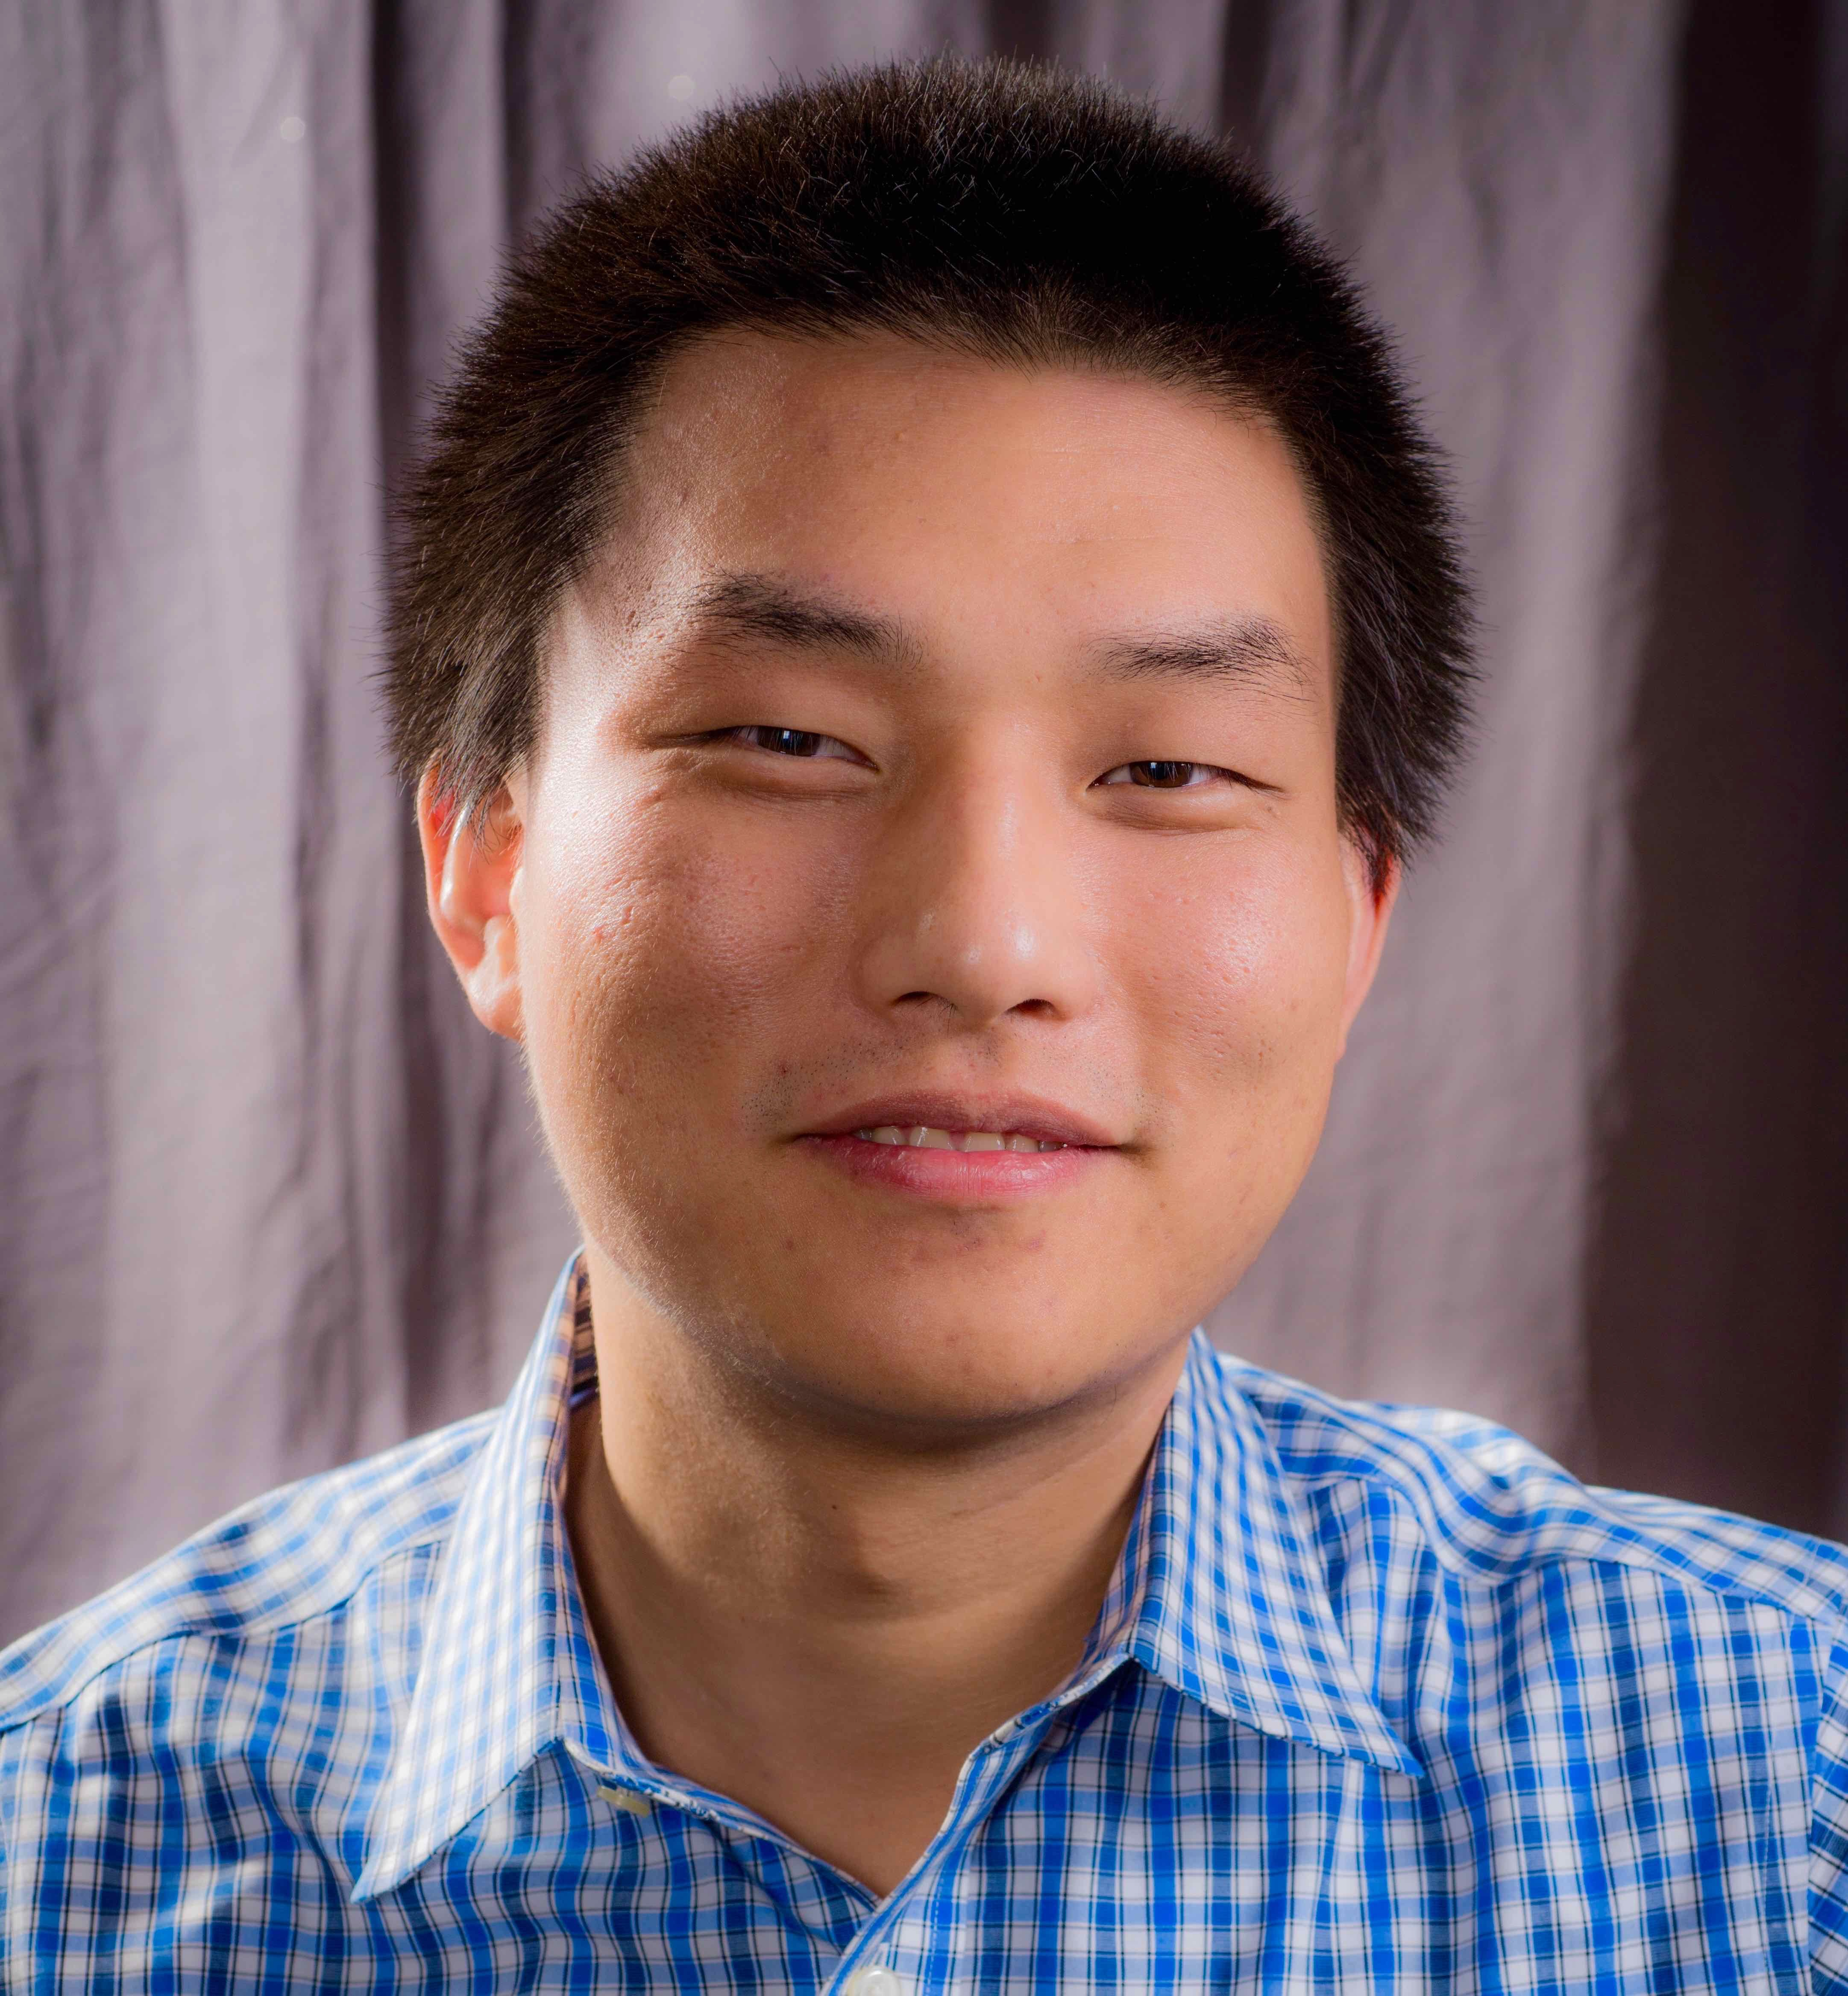
\includegraphics[width=\columnwidth]{lijun}
			\end{figure}
			\vspace{2mm}
			\begin{figure}
				\centering
				
\includegraphics[width=\columnwidth]{sams_logo}
			\end{figure}
		\end{column}
	\end{columns}
\end{frame}

\begin{frame}
	\frametitle{Outline}
	\tableofcontents[hideallsubsections]
\end{frame}

%-------------------------------------------------------------------------------
% Time series analysis basics
%-------------------------------------------------------------------------------
\section{Time series analysis}

\begin{frame}
	\frametitle{Time Series is Ubiquitous}
	\begin{columns}
		\begin{column}{0.4\linewidth}
			\begin{itemize}
				\item Time series record a history of states
					\begin{itemize}
						\item price hisory
						\item sales records
						\item sensor signal
						\item operational log
					\end{itemize}
				\item History is useful if it helps us make decisions
				\item Decision leads to business impact
			\end{itemize}
		\end{column}
		\hfill
		\begin{column}{0.6\linewidth}
			\begin{figure}
				\centering
				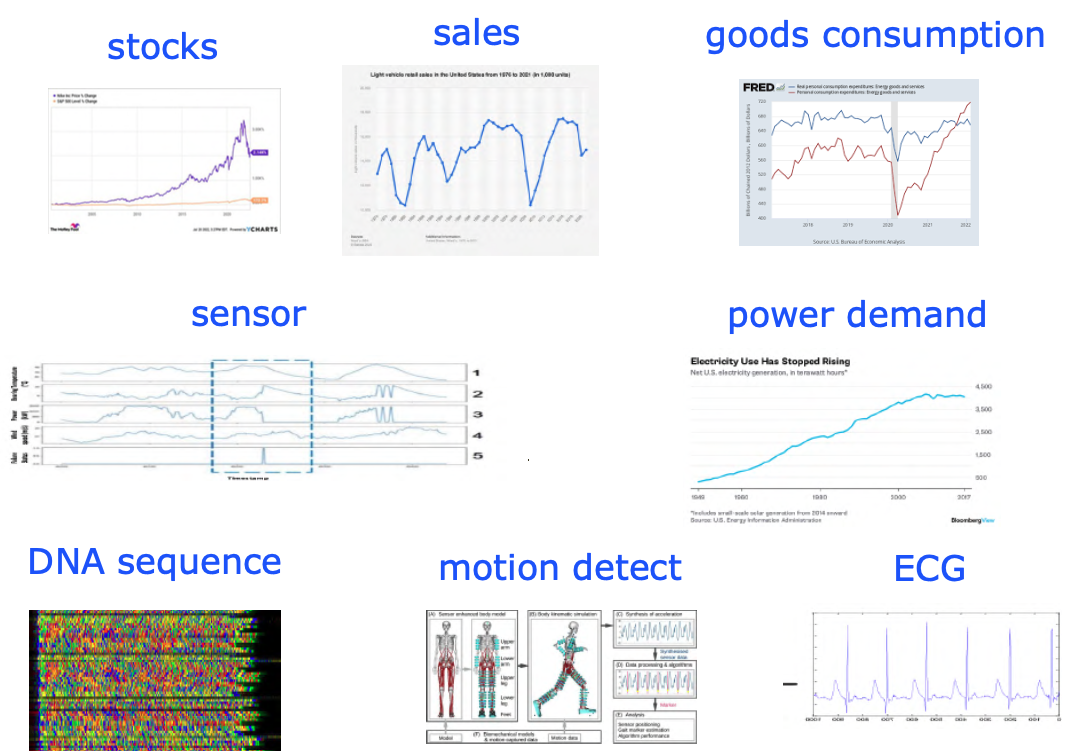
\includegraphics[width=\columnwidth]{time_series}
				\tiny{Image courtesy of \cite{wen2022robust}.}
			\end{figure}
		\end{column}
	\end{columns}
\end{frame}

\begin{frame}
	\frametitle{Typical Applications on Time Series}
	\begin{figure}
		\centering
		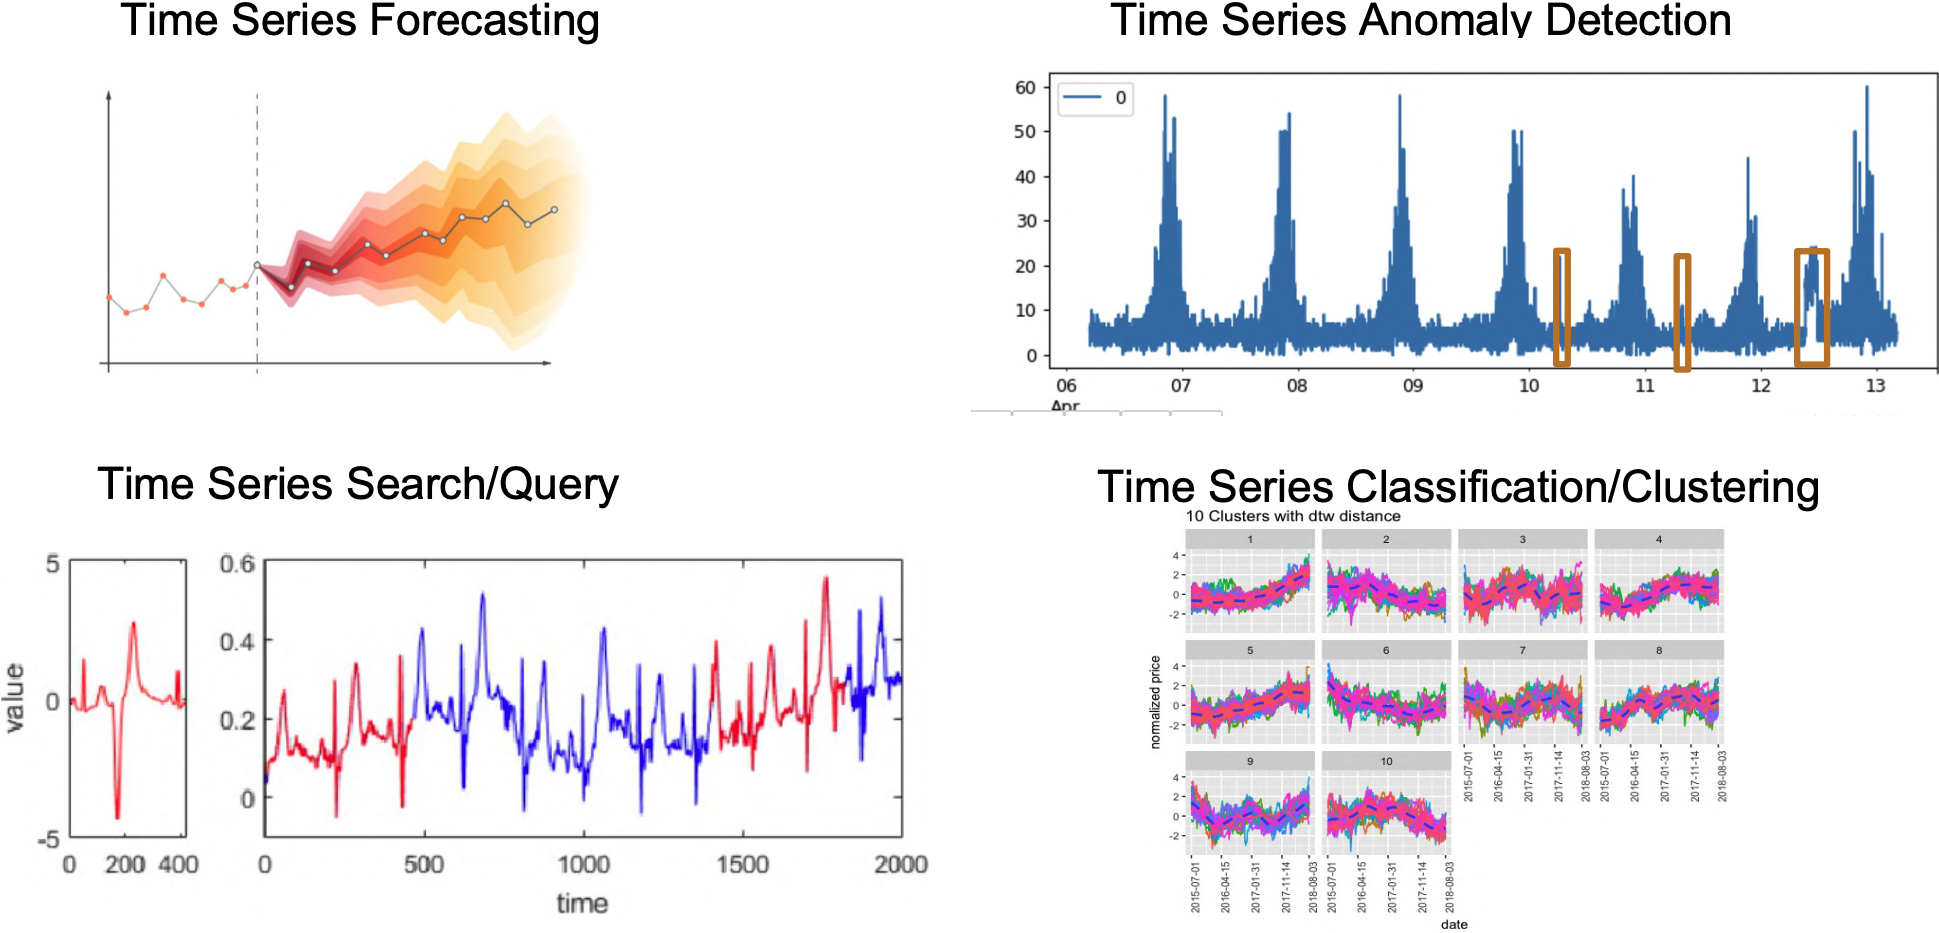
\includegraphics[width=\linewidth]{time_series_applications}
		\tiny{Image courtesy of \cite{wen2022robust}.}
	\end{figure}
\end{frame}

\begin{frame}
	\frametitle{From Forecast to Decision}
	\begin{itemize}
		\item Allocate resource based on demand forecast
		\item Peak demand vs. average demand
		\item Lead time and forecast horizon
	\end{itemize}
	\vfill
	\begin{figure}
		\centering
		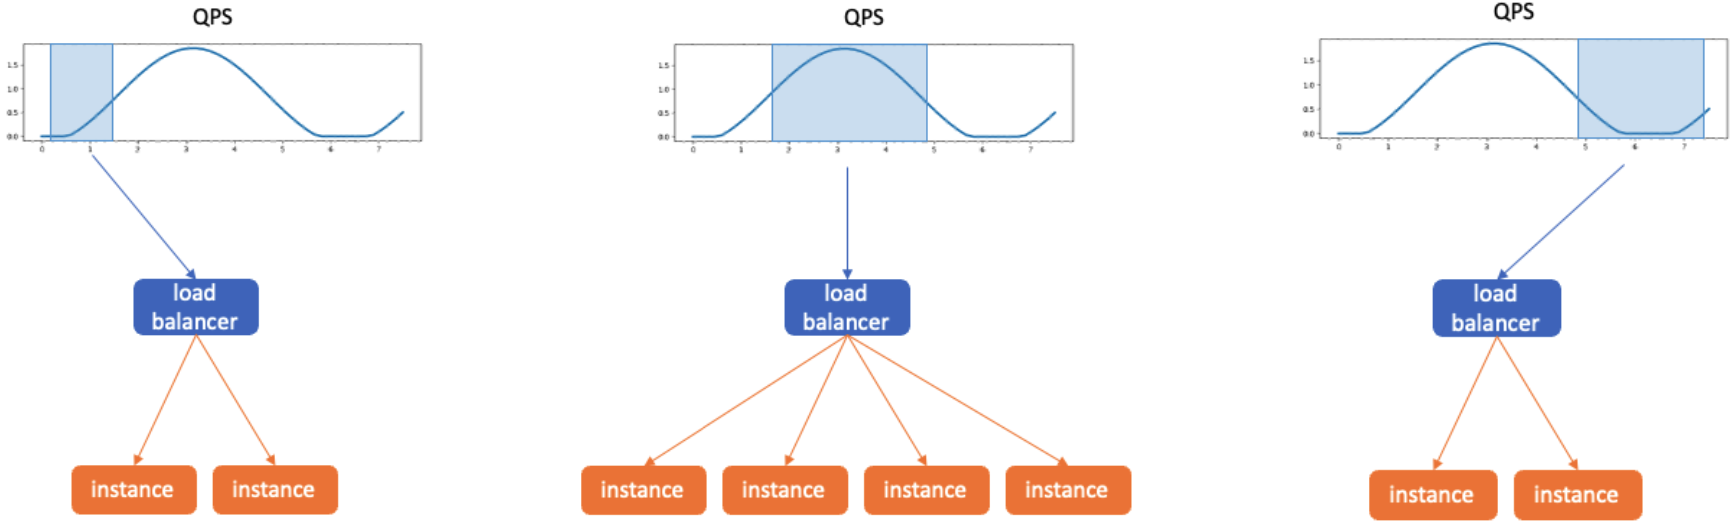
\includegraphics[width=\linewidth]{forecast}
		\tiny{Image courtesy of \cite{wen2022robust}.}
	\end{figure}
\end{frame}

\begin{frame}
	\frametitle{From Anomaly Detection to Cause Analysis}
	\begin{columns}
		\begin{column}{0.4\linewidth}
			\begin{figure}
				\centering
				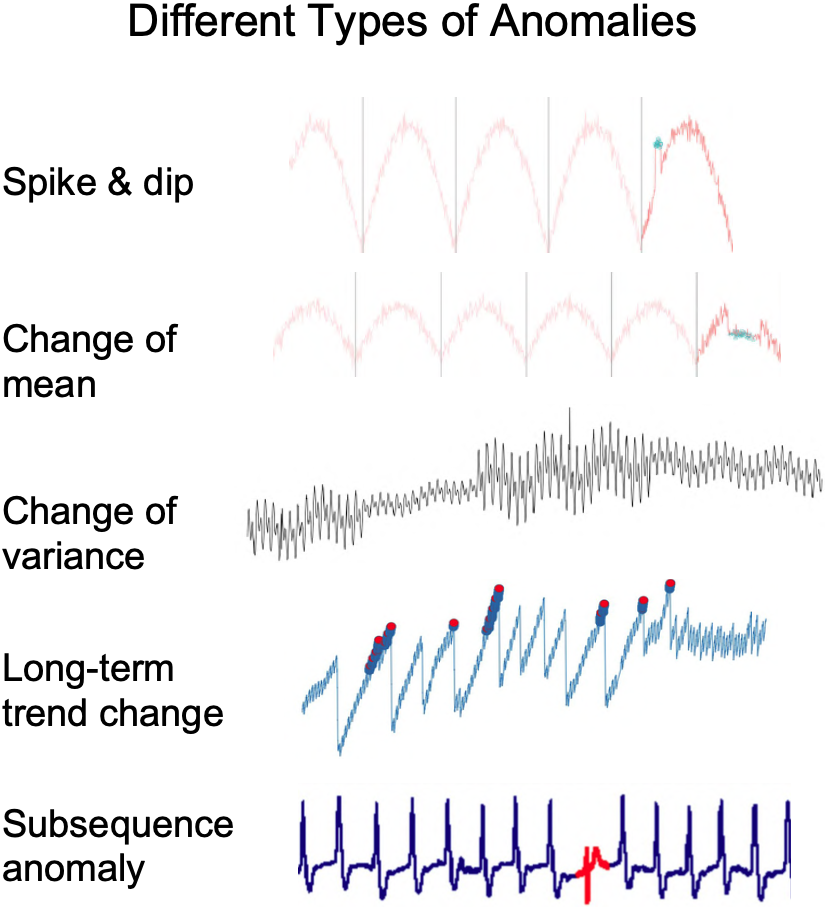
\includegraphics[width=\columnwidth]{anomaly}
			\end{figure}
		\end{column}
	\end{columns}
\end{frame}

%-------------------------------------------------------------------------------
% Industry perspective for campus hires
%-------------------------------------------------------------------------------
\section{Industry perspective}

%-------------------------------------------------------------------------------
% Q & A
%-------------------------------------------------------------------------------
\section{Q\&A}
\begin{frame}
	\center
	\Huge Q \& A
\end{frame}

\begin{frame}[t,allowframebreaks]
	\frametitle{References}
	\tiny
	\printbibliography
\end{frame}

\end{document}
